\section{Contributions}
%This thesis strives to showcase the usefulness of the neighborhood
%concepts and address the efficiency issues when adopting with
%nontrivial analytic functions. 
In brief, this thesis entitles a twofold contribution.
First, by sewing different $\mathcal{N}$s and $\mathcal{F}$s, 
several novel neighborhood queries are proposed for 
\emph{graph}, \emph{sequence data} and \emph{trajectory} domains respectively. 
%three interesting
%neighborhood analytic queries are proposed for \emph{graph}, \emph{time series} 
%and \emph{trajectory} domains respectively. 
Second, this thesis
deals with the efficiency issues in deploying the corresponding analytic queries to
handle data of nowadays scale.
The roadmap of this thesis is shown in Figure~\ref{fig:thesis_roadmap}.
\begin{figure}[h]
\centering
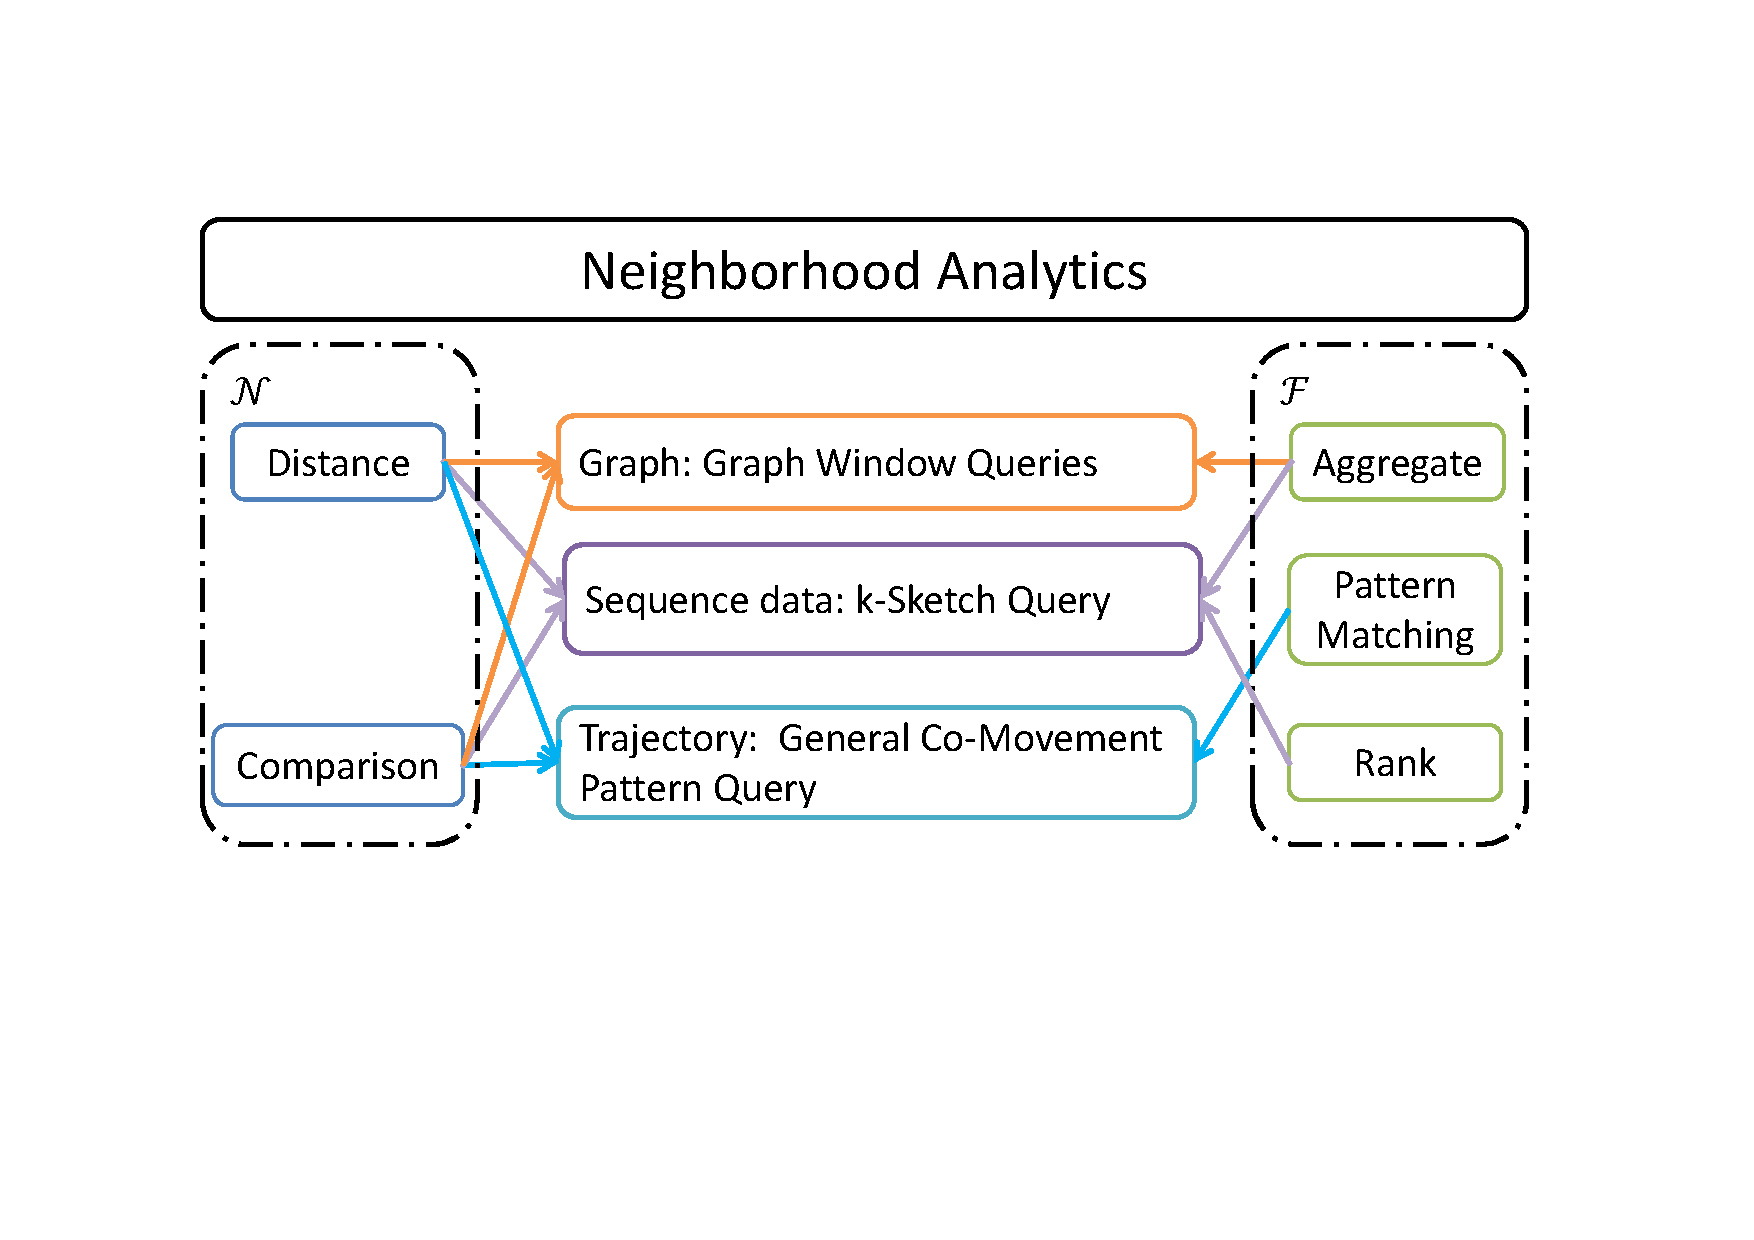
\includegraphics[width=0.8\linewidth]{thesis_roadmap.pdf}
\caption{The road map of this thesis. There are three major contributions as highlighted in the center. Each contribution
is a neighborhood analytic based on different $\mathcal{N}$ and $\mathcal{F}$ as indicated by arrows.} 
\label{fig:thesis_roadmap}
\end{figure}

In a nutshell, we propose the neighborhood queries in three data domains. 
In \emph{graph}, we identify two types of queries: \emph{k-hop window query} is based on the \emph{distance} neighborhood
and \emph{topological window query} is based on the \emph{comparison} neighborhood. 
In \emph{sequence data}, we propose a nested \emph{distant} and \emph{comparison} neighborhoods
query named $k$-Sketch to finding striking rank-aware streaks.
In \emph{trajectory}, we analyze existing movement patterns based
on \emph{distance} and \emph{comparison} neighborhoods and unify
the existing works with a general pattern discovery query. Next, we present our contributions in detail for each of the data domains.


\subsection{Window Queries for Graph Data}
The first piece of the thesis deals with neighborhood query
on graph data. Nowadays information network are typically
modeled as attributed graphs where the 
vertexes correspond to objects and the edges capture the
relationships between these objects. As vertexes embed a wealth
of information (e.g., user profiles in social networks), there are 
emerging demands on analyzing these data to extract useful insights. 
We propose the concept of \emph{window analytics} 
for attributed graph and identify two types of such analytics as shown in the following examples:

\begin{example}[$k$-hop window]
In a social network (such as Linked-In and Facebook etc.), users are normally modeled as vertexes and connectivity relationships are modeled as edges. In the social network scenario, it is of great interest to summarize the most relevant connections to each user such as the neighbors within $2$-hops. Some analytic queries such as summarizing the related connections' distribution among different companies, and computing age distribution of the related friends can be useful. In order to answer these queries, collecting data from every user's neighborhoods within 2-hop is necessary.
\end{example}
\begin{example}[Topological window]
In biological networks (such as Argocyc, Ecocyc etc.), genes, enzymes and proteins are vertexes and their
dependencies in a pathway are edges. Because these networks are directed and acyclic, 
in order to study the protein regulating process, one may be interested to find out the statistics of molecules in each protein production pathway. For each protein,we can traverse the 
graph to find every other molecules that are in the upstream of its pathway.
Then we can group and count the number of genes and enzymes among those molecules.
\end{example}

The two \emph{windows} shown in the examples are essentially neighborhood functions defined for each vertex. Specifically, let $G=(V:E:A)$ be an attributed graph, where $V$ is the set of vertexes, $E$ is the set of edges, and each vertex $v$ is associated as a multidimensional points $a_v \in A$ called attributes.
The \emph{k-hop} window is a \emph{distance} neighborhood function, 
i.e., $\mathcal{N}_1(v,k)= \{u|\mathtt{dist}(v,u) \leq k\}$, 
which captures the vertexes that are $k$-hop nearby. 
The \emph{topological} window,  $\mathcal{N}_2(v)= \{u | u \in v.ancestor\}$,
is a \emph{comparison} neighborhood function that captures
the ancestors of a vertex in a directly acyclic graph.  The analytic function $\mathcal{F}$ is an aggregate function (sum, avg, etc.) on $A$.

Apart from demonstrating the useful use-cases on these two windows, 
we also investigate on supporting efficient window processing.  We propose
two different types of indexes: Dense Block Index (DBIndex)
and Inheritance Index (I-Index). The DBIndex and I-Index
are specially optimized to support k-hop window and topological
window processing. These indexes
integrate the aggregation process with partial work sharing techniques
to achieve efficient computation.
In addition, we develop space-and-performance efficient techniques
for the index construction. Notably, DBIndex saves upto 80\%
of indexing time as compared to the state-of-the-art competitor and upto 10x
speedup in query processing. 


\subsection{$k$-Sketch Query on Time Sequenced Events}
The second piece of the thesis explores the neighborhood
query for time sequenced events. 
In time sequenced events analysis, an important
and revenue-generating task is to detect sensational patterns.
An outstanding neighborhood based pattern is the \emph{streak}~\cite{zhang2014discovering}. 
Streak has been found useful in many sequenced applications,
such as network monitoring, stock analysis
and sport reporting. For example, streaks may be of the following forms:
\begin{enumerate}
	\item{[STOCK]:``Apple Inc. has an average price of USD 115.5 in the last week''}
	\item{[SPORTS]: ``Kobe has scored at least 60 points in three straight games' }
\end{enumerate}
% in stock analysis,
%a streak could be ``Apple Inc. has an average price of USD 115.5 in the last week''.
%In computational journalism, a streak could be ``Kobe has scored at least 60 points in three straight games''.
Essentially, a \emph{streak} is constructed from two concepts: an \emph{aggregate function} (e.g., average, min)
applied on a \emph{time window} of events (e.g., seven days, three games).
%
%comprises of two elements: a time window of events (e.g., seven days, three games)
%and an aggregate function on the window (e.g., average, min). 
This makes the streak as a neighborhood query of events where the neighborhood function is defined as time windows.
%
%Since the streak is aggregated based on the
%closeness of events in the time domain (i.e., time window), it can be viewed as a neighborhood query where the neighborhood function is defined by the time distance, and the analytic function can be any aggregate function.

However, it is challenging to directly adopt streaks in discovering sensational patterns because
the strikingness of a streak is unknown.
%A direct challenge in discovering phenomenal patterns using streak is
%how to quantify the strikingness of a streak.
For example, \emph{Streak 1} would not be striking if all NBA players score over 60 points. 
On the contrary, knowing that NBA players in average only score 20 points, then \emph{Streak 1} is quite striking. 
To quantify the strikingness of a streak, we propose a \emph{rank-aware streak} that measures the strikingness of
a streak by comparing among all streaks under same condition (i.e., window length).

%
% 
%However, when analyzing the streak, the amount of streaks for a subject 
%is too huge (i.e., $O{N \choose 2}$ for a subject with $N$ data points) 
%to conduct effective analytics. 
%Observed that many streaks share almost identical information, we are motivated 
%to propose a $k$-Sketch
%query to effectively select $k$ most representative streaks.
%
%The $k$-sketch query is built on a core concept named \emph{rank-aware streak},
%out of which $k$ representatives are 
%chosen based on a novel scoring function
%that balances the strikingness and the diversity. A \emph{rank-aware streak}
%enriches traditional streak by including the
%relative position of a streak among its cohort.
%Such a concept is not rare in real-life.
%For example, journalists often adopt the rank-aware streak to promote
%the attractiveness of their news:

% For each subject,
%we then select $k$ \emph{rank-aware} streaks that best cover all
%data points of a subject with highest ranks called $k$-sketch.
%In real life,
%rank-aware streaks are often seen in journalism to promote the attractiveness
%of news.
%For example:
%We notice that many streaks share the same information which
%result in near-duplicate output. Therefore, we propose a $k$-Sketch
%query to effectively select $k$ most representative streaks.
%In modeling, we first enrich the semantic of stream 
%%We enrich the semantic of \emph{streak} 
%by proposing the \emph{rank-aware} streak, which computes the
%relative position of a streak among its cohort. In real-life,
%rank-aware streaks are often adopted to promote the attractiveness of news. For example:

%\eat{The second piece of the thesis proposes a neighborhood
%query in \emph{time series} domain to support the rank-aware streak discovery. 
%In time series domain, an 
%important and revenue generating tasks is to detect phenomenal patterns. However,
%as the large amount of the data stored and continuously generated, it is
%almost impossible for humans to manually detect these patterns. A prominent 
%example of such patterns is \emph{streak}, which refers to a subject is outstanding
%for consecutive events. We enhance the traditional \emph{streak} to incorporate with
%rank-awareness. Coincidentally, the \emph{rank-aware streak} are very prevalent
%in real life:}
%\eat{
%The second piece of the thesis proposes a neighborhood
%query to support automatic discovery of news in time series data.
%Nowadays events are collected in a timestamped format and journalists needs to manually synthesize those events to produce interesting news. We propose the automatic \emph{rank-aware news theme} detection with the aim to alleviate human efforts in poring over a large amount of data. 
%Coincidentally, the \emph{rank-aware news theme}s are very prevalent
%in real life new reporting:
%\begin{enumerate}
%\setlength\itemsep{-0.05cm}
%\item(Feb 26, 2003) With 32 points, Kobe Bryant saw his 40+ scoring streak end at \textbf{nine} games,  tied with Michael Jordan for \textbf{fourth} place on the all-time list\footnote{\url{http://www.nba.com/features/kobe_40plus_030221.html}}. 
%
%\item(April 14, 2014) Stephen Curry has made 602 3-pointer attempts from beyond the arc,... are the \textbf{10th} most in NBA history in a season (\textbf{82 games})\footnote{\url{http://www.cbssports.com/nba/eye-on-basketball/24525914/stephen-curry-makes-history-with-consecutive-seasons-of-250-3s}}.
%
%\item (May 28, 2015) Stocks gained for the \textbf{seventh consecutive day} on Wednesday as the benchmark moved close to the 5,000 mark for \textbf{the first} time in seven years\footnote{\url{http://www.zacks.com/stock/news/176469/china-stock-roundup-ctrip-buys-elong-stake-trina-solar-beats-estimates}}.
%
%\item (Jun 9,  2014) Delhi has been witnessing a spell of hot weather  over the \textbf{past month}, with temperature hovering around 45 degrees Celsius, .... \textbf{highest} ever since 1952\footnote{\url{http://www.dnaindia.com/delhi/report-delhi-records-highest-temperature-in-62-years-1994332}}.
%
%\item(Jul 22, 2011) Pelican Point recorded a maximum rainfall of 0.32 inches for \textbf{12 months}, making it the  \textbf{9th driest} places on earth\footnote{\url{http://www.livescience.com/30627-10-driest-places-on-earth.html}}.
%\end{enumerate} 
% 
%In the above examples, each news is a rank-aware streak consisting of five elements: a subject (e.g., Kobe Bryant, Stocks, Delhi), an event window (e.g., nine straight games, seventh consecutive days, past month), an aggregate function on an attribute
%(e.g., minimum points, count of gains, average of degrees), a rank (e.g., fourth, first time, highest), and a
%historical dataset (e.g., all time list, seven years, since 1952). These indicators are summarized in
%Table~\ref{tbl:news-example}.}

Technically, the rank-aware streak can be formally described using a joint neighborhood function. 
Let $e_s(t)$ denote the event of subject $s$ at time $t$. Then the rank-aware streaks are generated using neighborhood analytics in a two-step manner: 

(1) a \emph{distance neighborhood} $\mathcal{N}_1(o_i,w)=\{o_j | o_i.t - o_j.t \leq w \}$ groups a consecutive $w$ events for each event. Let $\overline{v}$ be the aggregate value associated with $\mathcal{N}_1$, then the output of this step is a set of \emph{event windows} of the form  $n=\langle o_i, w, t, \overline{v} \rangle$.

(2) a \emph{comparison neighborhood} $\mathcal{N}_2(n_i) = \{n_j | n_j.w = n_i.w \wedge n_i.\overline{v} \geq n_j.\overline{v} \}$ ranks a subject's event window among all other event windows with the same window size. The result of the this step is a tuple $\langle o_i, w, t, r \rangle$, where $r$ is the \emph{rank}.
%
% Technically,
%a rank-aware streak comprises of three part: the event window, the aggregate function and the \emph{rank}
%of the aggregate value under all events with the same window length. 

As the rank-aware streak contains the position of the streak among its cohort, we are able to
quantitative measure the strikingness based on the rank value. 
For example, the rank-aware
version of \emph{Streak 1} would be ``Kobe has scored at least 60 points in three straight games, which is best in the league''.  This clearly suggests that \emph{Streak 1} is striking.
%
%We can easily tell that \emph{rank-aware} streak help to provide the strikingness of a streak.  It is also 
%notable that the \emph{rank-aware} streak can be also modeled in a neighborhood way.

\eat{In the above news themes, there are a subject (e.g., Kobe Bryant, Stocks, Delhi), an event window (e.g., nine straight games, seventh consecutive days, past month), an aggregate function on an attribute
(e.g., minimum points, count of gains, average of degrees), a rank (e.g., fourth, first time, highest), and a
historical dataset (e.g., all time list, seven years, since 1952). These news theme indicators are summarized in Table~\ref{tbl:news-example}.  }


%\begin{table}[h]
%\centering
%\begin{tabular}{|c|c|c|c|c|}
%\hline
%\textbf{E.g.} & \textbf{Subject} & \textbf{Aggregate function} & \textbf{Event window} & \textbf{Rank} \\
%\hline
%1 & Kobe Bryant &$\mathtt{min}$(points) & 9 straight games & 4 \\
%\hline
%2 & Stephen Curry &$\mathtt{sum}$(shot attempts) & 82 games & 10 \\
%\hline
%3 & Stocks &$\mathtt{count}$(gains) & 7 consecutive days & 1 \\
%\hline
%4 & Delhi &$\mathtt{avg}$(degree) & past months (30 days) & 1 \\
%\hline
%5 & Pelican Point &$\mathtt{max}$(raindrops) & 12 months & 9 \\
%\hline
%\end{tabular}
%\caption{News theme summary}
%\label{tbl:news-example}
%\end{table}

%\revised{We model these rank-aware streaks using nested neighborhood analytics.}
\eat{We model these news themes using nested neighborhood analytics.
Let $e_s(t)$ denote the event of subject $s$ at time $t$. Then the rank-aware streaks are generated using neighborhood analytics in a two-step manner: 

(1) a \emph{distance neighborhood} $\mathcal{N}_1(o_i,w)=\{o_j | o_i.t - o_j.t \leq w \}$ groups a consecutive $w$ events for each event. Let $\overline{v}$ be the aggregate value associated with $\mathcal{N}_1$, then the output of this step is a set of \emph{event windows} of the form  $n=\langle o_i, w, t, \overline{v} \rangle$.

(2) a \emph{comparison neighborhood} $\mathcal{N}_2(n_i) = \{n_j | n_j.w = n_i.w \wedge n_i.\overline{v} \geq n_j.\overline{v} \}$ ranks a subject's event window among all other event windows with the same window size. The result of the this step is a tuple $\langle o_i, w, t, r \rangle$, where $r$ is the \emph{rank}.}

%It is easy to verify that $\mathcal{N}_2 \cdot \mathcal{N}_1$ result in the rank-aware streaks.
% is the \emph{rank-aware news themes}. Rooted from the \emph{rank-aware news themes}, we further address the problem 
%of controlling the result size.
%We propose
%a novel concept named \emph{Sketch} to avoid outputting near-duplicate themes.
%A sketch contains $k$ most representative rank-aware news themes under a scoring function that considers both strikingness and diversity.  Our objective is to discover sketches for each subject in the domain.


Another challenge in the pattern discovery is that the amount of streaks
for a subject is huge. For a subject with $N$ events,
there are $O{N\choose 2}$ streaks as well as rank-aware streaks. 
In real life, ``Kobe'' has played $1000$ games which introduces near half million streaks.
Such a large number poses difficulties for selecting phenomenal streaks. 
We observe that many streaks share almost identical information. For example, Kobe has scored 81 points
in one game. This single-event streak ranks number 1 among all streaks. Subsequently, Kobe has
scored an average of 47 points for 2 straight games, which is only ranked number 10. Therefore, reporting
the second streak does not provide additional information for the total sketch query.
Based on this observation, we
propose a $k$-Sketch query to effectively select the $k$ most \emph{representative streaks}.
%
%Our $k$-Sketch query is based on a novel scoring function that consider both the 
%stringness and the diversity of the streaks. 

In this thesis, we further study
the technical issues in running $k$-Sketch queries in both online and offline scenarios.
%
%
%Besides proposing the rank-aware streak, we also technically 
%study how to efficiently support the \emph{$k$-Sketch} query in both
%offline and online scenarios. We propose various window-level 
%pruning techniques to find striking candidate steaks.
%Among those candidates, we then develop approximation
%methods, with theoretical bounds, to discover $k$-sketches for each subject. 
Lastly, we conduct experiments on four real
datasets, and the results demonstrate the efficiency and 
effectiveness of our proposed algorithms: the running time
achieves up to 500x speedup as compared to baseline and the quality of the
detected sketch is endorsed by the anonymous users
from Amazon Mechanical Turk \footnote{\url{https://requester.mturk.com}}.

\subsection{Co-Movement Pattern Query in Trajectory Data}
The third piece of the thesis studies the neighborhood
query on the trajectory domain. 
In the trajectory domain, an important
mining task is to discover traveling patterns among moving objects.
A \emph{co-movement pattern}~\cite{li2013managing,zheng2015trajectory} is a popularly studied movement pattern
which refers to a group of moving objects traveling together for a certain 
period of time. A pattern is prominent if the group 
size exceeds $M$ and the length of duration exceeds $K$. 
The group is defined based on the spatial proximity of objects, which 
can be seen as the spatial neighbors of the objects.
Rooted from the basic movement definition and driven by different mining applications,
there are several instances of co-movement patterns that have been developed with more advanced constraints.

Table~\ref{tbl:intro-move-patterns} summarizes several popular co-movement patterns with different 
constraints with respect to clustering in spatial proximity, consecutiveness in temporal duration
and computational complexity. In particular, the flock~\cite{gudmundsson2006computing} and the group~\cite{wang2006grouppattern} patterns require all the objects in a group to be enclosed by a disk with radius $r$;
whereas the convoy~\cite{jeung2008discovery}, the swarm~\cite{li2010swarm} and the platoon~\cite{li2015platoon} patterns resort to density-based spatial clustering. In the temporal dimension,
the flock~\cite{gudmundsson2006computing} and the convoy~\cite{jeung2008discovery} require all the timestamps
of each detected spatial group to be consecutive, which is referred to as global consecutiveness; whereas the swarm~\cite{li2010swarm} does not impose any restrictions. 
The group~\cite{wang2006grouppattern} and the platoon~\cite{li2015platoon} adopt 
a compromised approach by allowing arbitrary gaps between consecutive segments, 
which is called local consecutiveness. They introduce a parameter $L$ to control the minimum length of each local consecutive segment.


\begin{table}[h]
\centering
\begin{tabular}{|l|c|c|}
\hline 
\textbf{Pattern} & {\textbf{Proximity}} & { \textbf{Consecutiveness}} \\% & { \textbf{Time  Complexity}}\\ 
\hline 
flock~\cite{gudmundsson2006computing} & disk based &  global \\%& {$O(|\mathbb{O}||\mathbb{T}|\log(|\mathbb{O}|))$} \\ 
\hline 
convoy~\cite{jeung2008discovery} & density based &   global \\%& {$O(|\mathbb{O}|^2+|\mathbb{O}||\mathbb{T}|)$}\\ 
\hline 
swarm~\cite{li2010swarm} & density based  & - \\%& {$O(2^{|\mathbb{O}|}|\mathbb{O}||\mathbb{T}|)$}  \\ 
\hline 
group~\cite{wang2006grouppattern} & disk based &  local \\%& {$O(|\mathbb{O}|^2|\mathbb{T}|)$}\\ 
\hline 
platoon~\cite{li2015platoon} & density based &  local \\%& {$O(2^{|\mathbb{O}|}|\mathbb{O}||\mathbb{T}|)$}\\ 
\hline 
\end{tabular} 
\caption{Constraints of co-movement patterns.}
\label{tbl:intro-move-patterns}
\end{table}
%Neighborhoods relationship
%among moving objects forms the traveling behavior of the objects
%which is often referred as moving patterns. Specifically, the neighborhoods
%of objects are defined based on the spatial proximity and the 
%
%
%nIn trajectory domain, an instance 
%of neighborhood usage is to detect the movement pattern. In simple
%words, a movement pattern is a set of moving object whose trajectories
%exhibits interesting behaviors.
%
%Due to its wide spectrum of applications, 
%mining the movement patterns have attracted many research attention.

%
%In trajectory domain, the neighborhoods of objects across multiple time snapshots collectively 
%form a movement pattern. Due to its wide spectrum of applications, mining the movement patterns have attracted many research attention.
%
%In the trajectory domain, neighborhood
%functions can effectively model the movement patterns
%of objects which is useful in a wide
%spectrum of applications. 
%
%An important mining task in trajectory
%data that has drawn many research attention is discovering
%movement patterns. Coincidentally, a movement pattern
%can be 
%
%
%Discovering co-movement patterns from large-scale trajectory 
%databases is an important mining task and has a wide
%spectrum of applications. 
%Existing studies have identified several types of interesting movement patterns called \emph{co-movement} patterns. A co-movement pattern refers to a group of moving objects traveling together for a certain period of time and the group of objects is normally determined by their spatial proximity. A pattern is prominent if the group size exceeds $M$ and the length of duration exceeds $K$. 
%Inspired by the basic definition 
%and driven by different mining applications, there are a bunch of variant 
%co-movement patterns that have been developed with more advanced constraints.

%\begin{figure}[h]
%\centering
%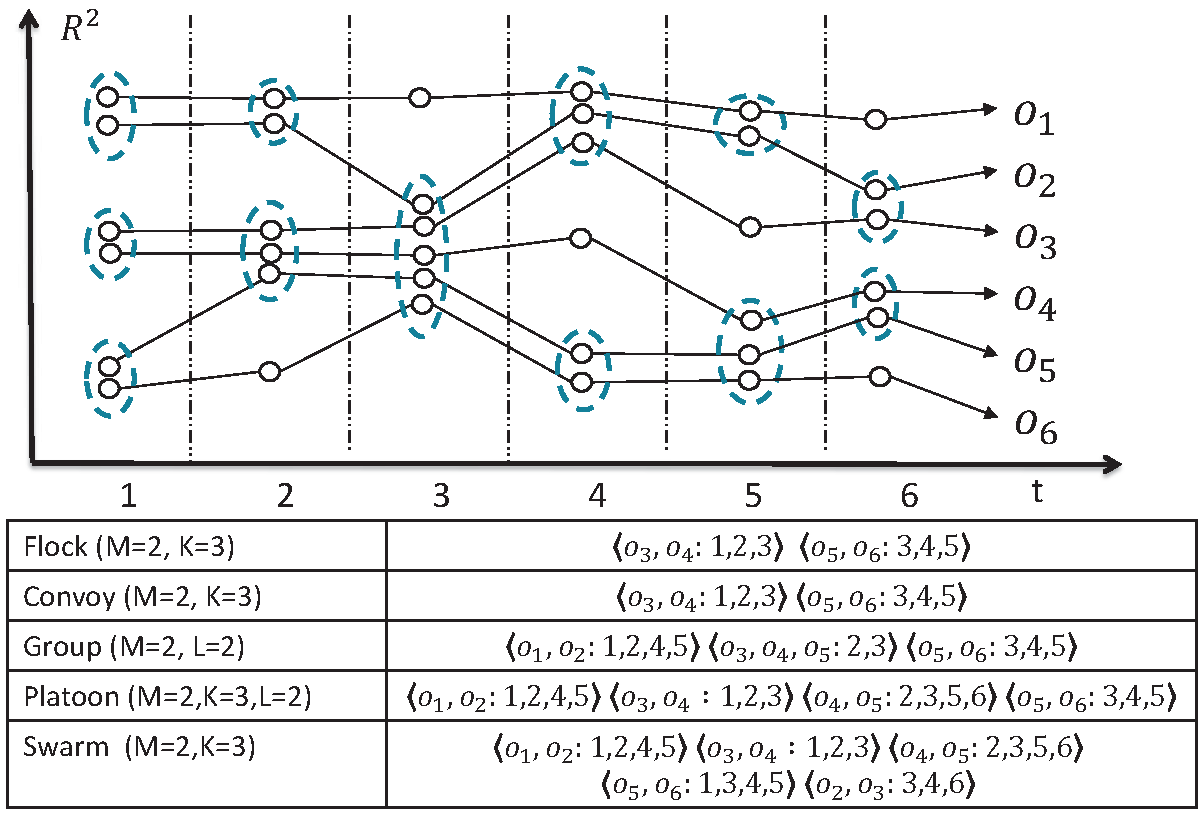
\includegraphics[width=0.8\textwidth]{trajectory_patterns.pdf}
%\caption{Trajectories and co-movement patterns. The example consists of six trajectories across six snapshots. Objects in spatial clusters are enclosed by dotted circles. $M$ is the minimum cluster cardinality; $K$ denotes the minimum number of snapshots for the occurrence of a spatial cluster; and $L$ denotes the minimum length for local consecutiveness.}
%\label{fig:related_work}
%\end{figure}
%
%Figure~\ref{fig:related_work} is an example to demonstrate the concepts of various co-movement patterns. The trajectory database consists of six moving objects and the temporal dimension is discretized into six snapshots. In each snapshot, we treat the clustering method as a black-box and assume that they generate the same clusters. Objects in proximity are grouped in the dotted circles. As aforementioned, there are three parameters to determine the co-movement patterns and the default settings in this example are $M=2$, $K=3$ and $L=2$. Both the \emph{flock} and the \emph{convoy} require the spatial clusters to last for at least $K$ consecutive  timestamps. Hence,$\langle o_3,o_4:1,2,3 \rangle$ and $\langle o_5,o_6:3,4,5 \rangle$  remains the only two candidates matching the patterns. The \textit{swarm} relaxes the pattern matching by discarding the temporal consecutiveness constraint. Thus, it generates many more candidates than the \textit{flock} and the \textit{convoy}. The \textit{group} and the \textit{platoon} add another constraint on local consecutiveness to retain meaningful patterns. For instance, $\langle o_1,o_2:1,2,4,5 \rangle$ is a pattern matching local consecutiveness because timestamps $(1,2)$ and $(4,5)$ are two segments with length no smaller than $L=2$. The difference between the \textit{group} and the \textit{platoon} is that the \textit{platoon} has an additional parameter $K$ to specify the minimum number of snapshots for the spatial clusters. This explains why $\langle o_3,o_4,o_5:2,3 \rangle$ is a \textit{group} pattern but not a \textit{platoon} pattern.


As shown, there are various types of co-movement patterns facilitating different application needs and it is cumbersome to deploy and optimize each of the pattern discovery algorithms. Therefore, it calls for a general framework to provide versatile and efficient support of all these pattern discoveries. We observe that 
these co-movement patterns can be uniformly represented as a two-step neighborhood query as follows:
	(1) $\mathcal{N}_1$ is a \emph{distance neighborhood} used to determine the spatial proximity of objects. For example,  flock and group patterns uses the \emph{disk-based} clustering, which is equivalent to $\mathcal{N}_1(o_i)= \{o_j | \mathtt{dist}(o_i,o_j) < r \}$ for each object. Convoy, swarm and platoon patterns uses the \emph{density-based} clustering, which is equivalent to $\mathcal{N}_1(o_i)= \{o_j | \mathtt{dist}(o_j,o_k) \leq \epsilon \wedge o_k \in \mathcal{N}_1(o_i)\}$.
	(2) $\mathcal{N}_2$ is a comparison neighborhood used to determine the temporal constraints, i.e., $\mathcal{N}_2(o_i)=\{o_j, T | \forall t \in T, C_t(o_i) \equiv C_t(o_j)\}$, where $C_t(\cdot)$ returns the neighborhoods (i.e., $N_1$) of an object at time $t$.

Enlightened by the neighborhood unification, we propose a \emph{General Co-Movement Pattern} (GCMP)
query to capture all existing co-movement patterns. In GCMP, we treat the proximity detection (i.e., $\mathcal{N}_1$) as
a black box and only focus on the pattern detection (i.e., $\mathcal{N}_2$). It is notable that the GCMP
query is able to detect any of the existing co-movement patterns by adopting different analytic functions.



On the technical side, we study how to efficiently processing GCMP in a MapReduce platform to gain scalability for large-scale trajectory databases. In particular, we propose two parallel frameworks: (1) TRPM, which partitions trajectories by replicating snapshots in the temporal domain. Within each partitions, a line-sweep method is developed to find all patterns. (2) SPARE, which partitions trajectories based on object's neighborhood. Within each partitions, a variant of Apriori enumerator is applied to generate all patterns. We then show the efficiency of both our methods in the Apache Spark platform with three real trajectory datasets upto 170 million points. The results show that SPARE achieves upto 14 times efficiency as compared to TRPM, and 112 times speedup as compared to the state-of-the-art centralized schemes.